\chapter{Diseño e implementación} % Main chapter title

\label{Chapter3} % Change X to a consecutive number; for referencing this chapter elsewhere, use \ref{ChapterX}



En este capítulo se presentan los detalles del diseño de los nodos sensores y actuadores que conforman el trabajo, como así también los de la implementación de la aplicación Thingsboard.

\section{Arquitectura de la solución}
\label{sec:Arquitectura de la solución}

%Como se observa en la figura \ref{fig:blockdiagram}, el invernadero inteligente está compuesto por un conjunto de subsistemas encargados de las diferentes funciones de medición y control de variables, una aplicación central y un sistema que permita el acceso remoto de forma segura.

Para la implementación del prototipo propuesto en el trabajo se requirió la construcción de diferentes subsistemas encargados de las múltiples funciones dentro del invernadero inteligente. En forma general, cada uno de estos módulos opera en forma independiente del resto y se comunican por medio de una red inalámbrica con una aplicación central. 

Para garantizar el acceso de los usuarios desde Internet se desarrolló una interfaz segura que no involucra costos al cliente y no requiere cambios de configuración en su red hogareña.

En la figura \ref{fig:blockdiagram} se observa la arquitectura diseñada con los subsistemas implementados.


\begin{figure}[h]
	\centering
	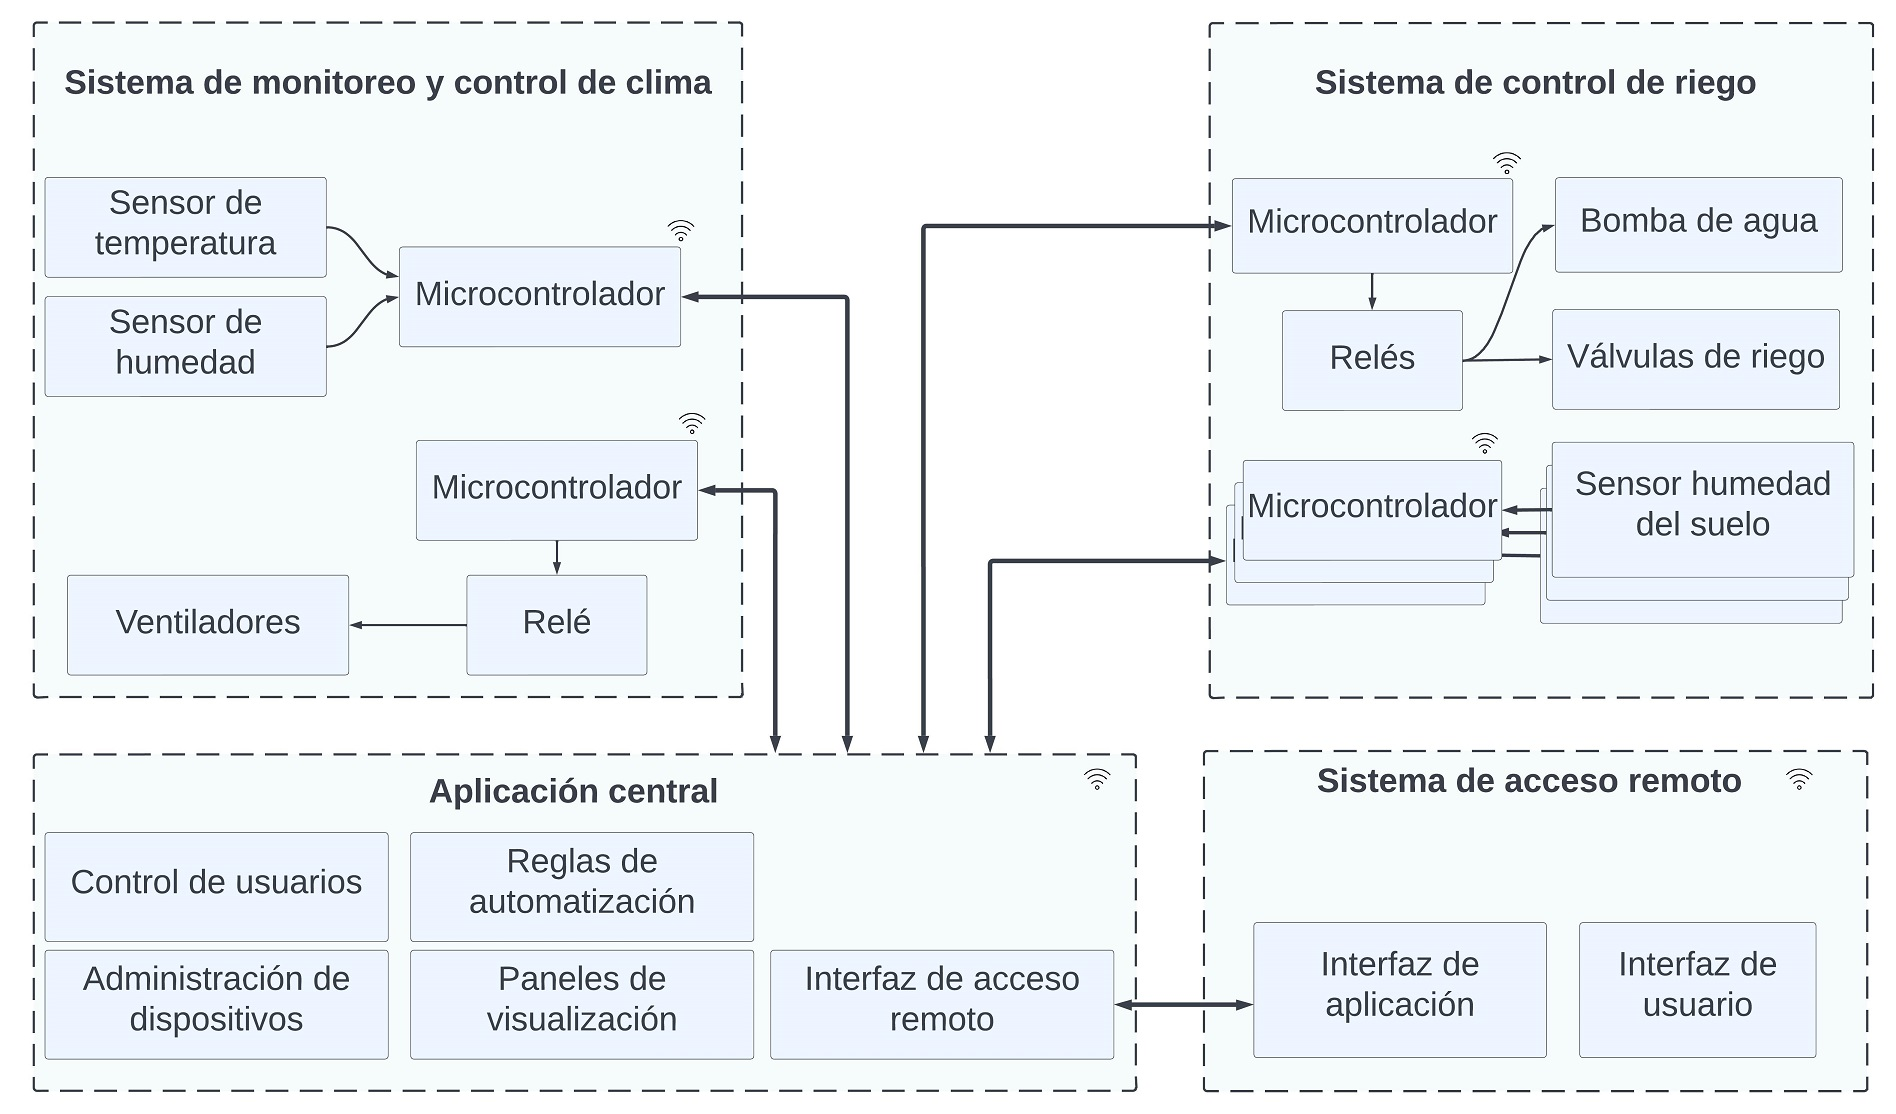
\includegraphics[width=1.0\textwidth]{./Figures/blockdiagram4.jpg}
	\caption[Arquitectura del sistema.]{Arquitectura del sistema.}
	\label{fig:blockdiagram}

\end{figure}

\subsection{Detalle de los sistemas}
\label{Detalle de los sistemas}

A continuación se detallan los subsistemas implementados en el trabajo:

\begin{itemize}
\item Sistema de monitoreo y control de clima: es responsable de medir la temperatura y humedad ambiente en el invernadero y enviar estas variables a la aplicación central. En base a los valores recibidos, la aplicación determina si es necesario enviar la señal de encender los ventiladores al microcontrolador correspondiente, y generar una alerta de aviso a los usuarios.


%
%\item Módulo de monitoreo de clima: es responsable de sensar la temperatura y humedad ambiente en el invernadero y enviar estas variables a la aplicación central para determinar las acciones a tomar en cuanto al control del clima.

\item Sistema de control de riego: está compuesto por múltiples sensores de humedad de suelo con sus respectivos microcontroladores que se distribuyen conforme a los circuitos de riego configurados. Los sensores proceden a enviar las mediciones a la aplicación central en donde se procesan los valores y en caso de ser necesario se dispara la señal de encendido a la válvula del circuito que corresponda, y luego a la bomba de agua para así comenzar el riego. Al mismo tiempo, el usuario recibe un alerta de accionamiento de la bomba.

\item Aplicación Central: constituye el cerebro del invernadero y es la encargada de almacenar los parámetros de configuración de los diversos sensores y actuadores, procesar los mensajes recibidos, disparar acciones y alertas y visualizar el estado general.

\item Sistema de acceso remoto: permite el acceso de usuarios a reportes del sistema en forma segura desde Internet.   
\end{itemize}

\subsection{Protocolos de comunicación}
\label{Protocolos de comunicación}
\textit{Aquí se describe cómo se comunican los sistemas con la aplicación central y los protocolos usado en cada caso.}

En la selección del software a emplear para la aplicación central se contempló qla compatibilidad con múltiples protocolos de comunicación. Sin embargo ciertas limitaciones de configuración específicas, tal como retención de los mensajes en las colas de MQTT, forzaron el utilizar diferentes protocolos dependiendo del módulo en cuestión. Otro factor condicionante, como se detalla en la sección \ref{sec:Ciberseguridad del sistema}, fue el carecer de una CA que emita certificados que todos los componentes puedan confiar.
En la figura \ref{fig:blockprotos} se ilustran los diferentes protocolos usados y cada caso de uso. 

\begin{figure}[h]
	\centering
	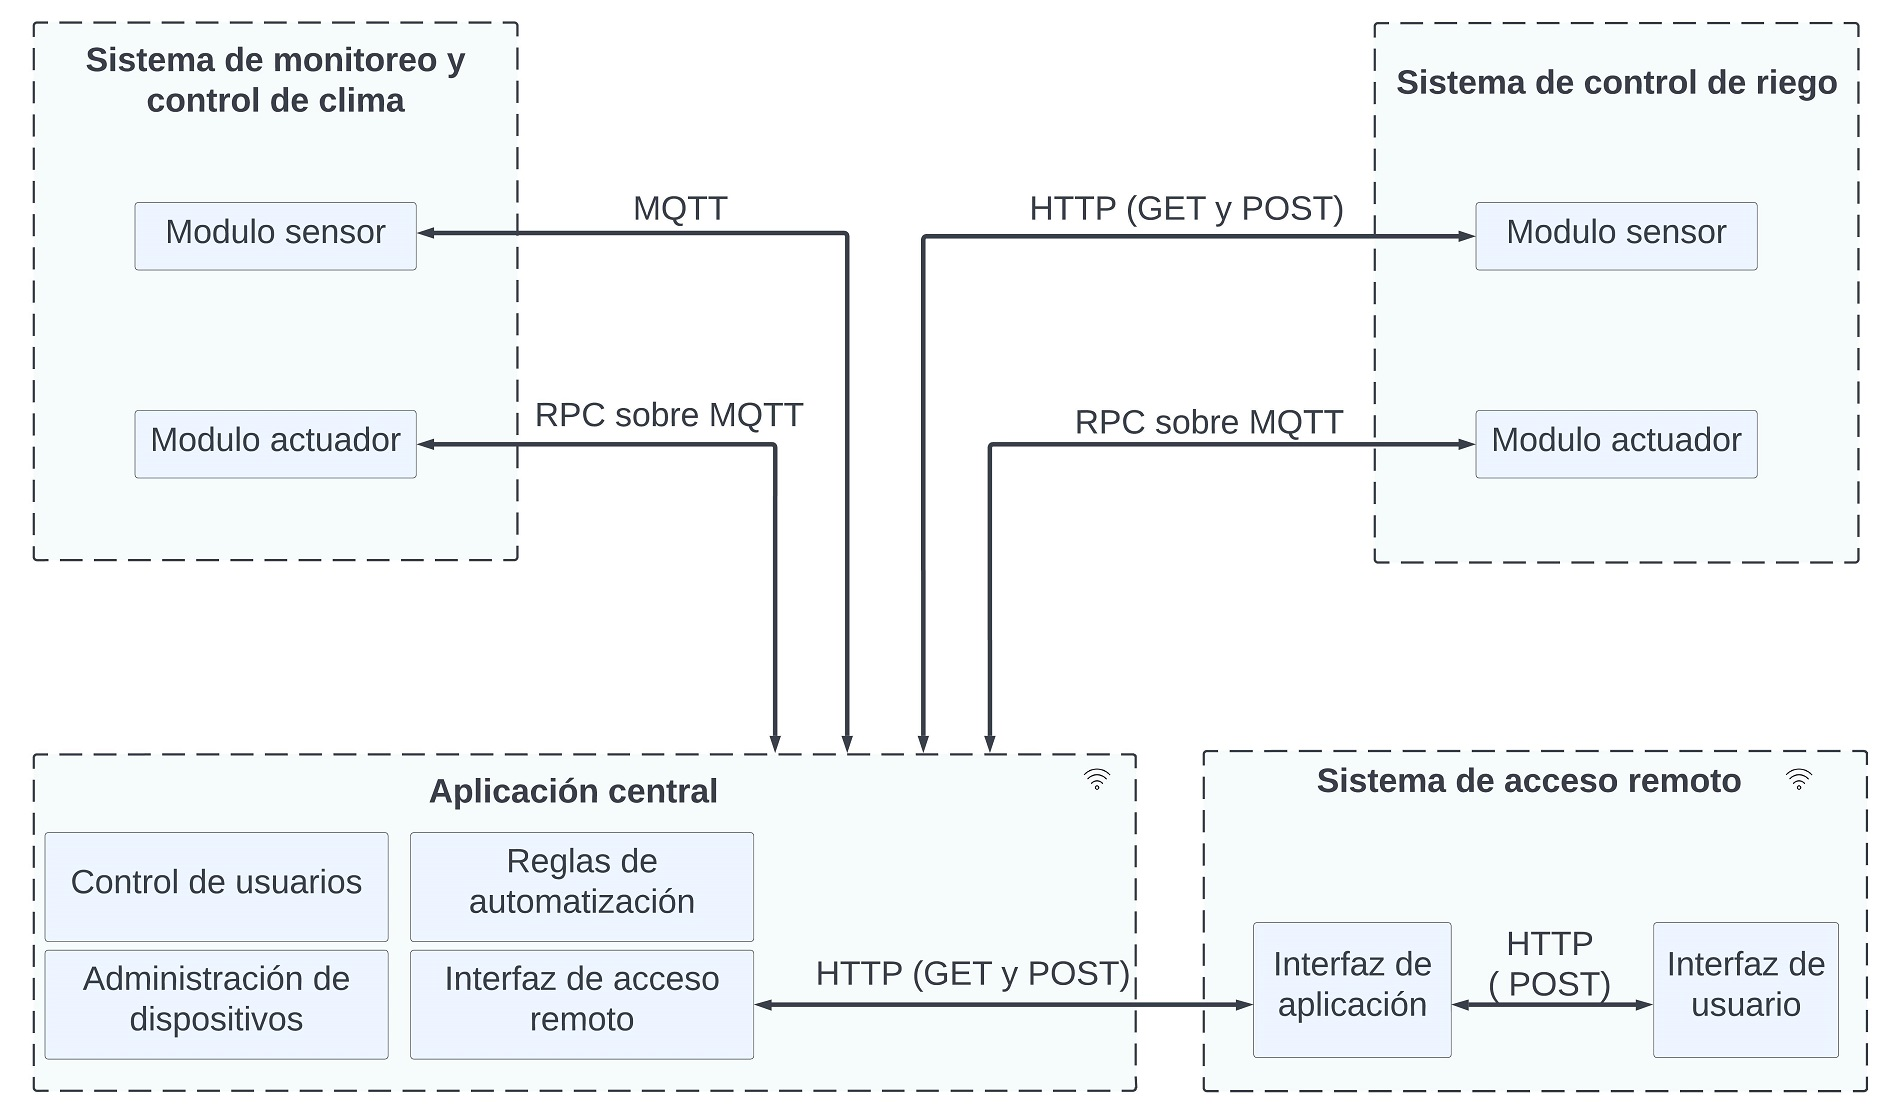
\includegraphics[width=1.0\textwidth]{./Figures/blockproto.jpg}
	\caption[Protocolos de comunicación entre módulos.]{Protocolos de comunicación entre módulos.}
	\label{fig:blockprotos}

\end{figure}

\section{Detalle de los módulos de hardware}
\label{sec:Módulos de hardware}

\subsection{Módulos sensores de humedad del suelo}
\label{Módulos sensores de humedad del suelo}

\subsection{Módulos controladores de riego}
\label{Módulos controladores de riego}

\subsection{Módulos sensores de temperatura y humedad}
\label{Módulos sensores de temperatura y humedad}

\subsection{Módulos controladores de clima}
\label{Módulos controladores de clima}

\section{Detalle del firmware desarrollado}
\label{sec:Desarrollo del firmware}

o:

\subsection{Programación del microcontrolador de medición de clima}
\label{Módulos controladores de clima}

\section{Detalle del firmware desarrollado}
\label{sec:Desarrollo del firmware}


\section{Selección y configuración del software}
\label{sec:Selección y configuración del software}

\section{Ciberseguridad del sistema}
\label{sec:Ciberseguridad del sistema}
